\documentclass[12pt]{report}
\renewcommand{\familydefault}{\sfdefault}
\usepackage[utf8]{inputenc}
\usepackage{fullpage}
\usepackage[english]{babel}
\usepackage{amsmath,amssymb}
\usepackage{graphicx}
\usepackage{cite}
\usepackage{fullpage}
\usepackage{tikz}
\usetikzlibrary{automata,arrows,positioning,calc}
\usepackage{caption}
\usepackage{natbib}
\usepackage{subfig}
\usepackage{caption}
\usepackage{titlesec, blindtext, color}
\definecolor{gray75}{gray}{0.75}
\newcommand{\hsp}{\hspace{20pt}}
\titleformat{\chapter}[hang]{\Huge\bfseries}{\thechapter\hsp\textcolor{gray75}{|}\hsp}{0pt}{\Huge\bfseries}

\usepackage{xcolor}
\colorlet{col1}{rgb:red,90;green,230;blue,129}
\colorlet{col2}{rgb:red,115;green,101;blue,230}
\colorlet{col3}{rgb:red,164;green,230;blue,78}
\colorlet{col4}{rgb:red,230;green,33;blue,33} 
\colorlet{col5}{rgb:red,230;green,207;blue,67}


\colorlet{c1}{col1!60}
\colorlet{c2}{col2!60}
\colorlet{c3}{green!60}
\colorlet{c4}{red}
\colorlet{c5}{yellow!60}
\colorlet{c6}{orange!70}
\colorlet{c7}{brown!70}
\colorlet{c8}{black!60}
\begin{document}


\begin{figure}[!h]
\centering
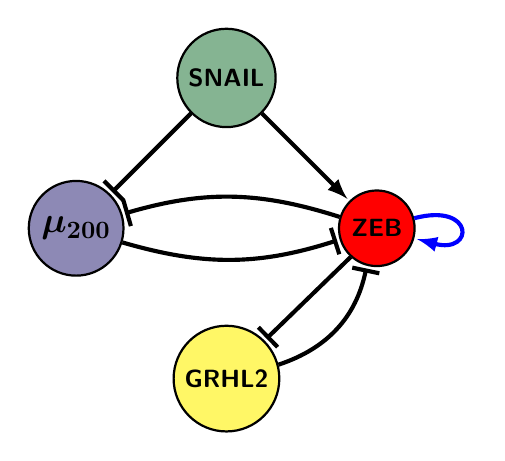
\begin{tikzpicture}[-|, >=stealth', auto, semithick, node distance=3cm,line width = 1.5pt]
\tikzstyle{every state}=[fill=white,draw=black,thick,text=black,scale=0.9]
\node[state, fill=c1]    (snail)                     {\textbf{SNAIL}};
\node[state, fill=c2]    (miR200) [below left of =snail] {\Large{$\boldsymbol{\mu_{200}}$}};
\node[state, fill=c4]    (ZEB)[below right of=snail]   {\textbf{ZEB}};
\node[state, fill=c5] (OVOL) [below left of=ZEB] {\textbf{GRHL2}};
\draw[
    >=latex,
%   every node/.style={above,midway},% either
    auto=right,                      % or
    loop above/.style={out=75,in=105,loop},
    every loop,
    ]
(snail) [-|] edge (miR200)
(snail) [->]edge  (ZEB)
(ZEB) [-|]edge[bend right=17]      (miR200)
(ZEB) edge[loop right, blue] (ZEB)
(OVOL) [-|]edge [bend right] (ZEB)
(ZEB) [-|] edge  (OVOL)
(miR200) [-|]edge [bend right=17] (ZEB);
\end{tikzpicture}

\end{figure}

\begin{figure}[!h]
\centering
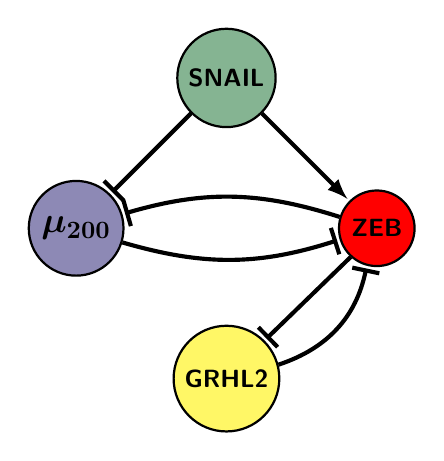
\begin{tikzpicture}[-|, >=stealth', auto, semithick, node distance=3cm,line width = 1.5pt]
\tikzstyle{every state}=[fill=white,draw=black,thick,text=black,scale=0.9]
\node[state, fill=c1]    (snail)                     {\textbf{SNAIL}};
\node[state, fill=c2]    (miR200) [below left of =snail] {\Large{$\boldsymbol{\mu_{200}}$}};
\node[state, fill=c4]    (ZEB)[below right of=snail]   {\textbf{ZEB}};
\node[state, fill=c5] (OVOL) [below left of=ZEB] {\textbf{GRHL2}};
\draw[
    >=latex,
%   every node/.style={above,midway},% either
    auto=right,                      % or
    loop above/.style={out=75,in=105,loop},
    every loop,
    ]
(snail) [-|] edge (miR200)
(snail) [->]edge  (ZEB)
(ZEB) [-|]edge[bend right=17]      (miR200)
(OVOL) [-|]edge [bend right] (ZEB)
(ZEB) [-|] edge  (OVOL)
(miR200) [-|]edge [bend right=17] (ZEB);
\end{tikzpicture}

\end{figure}

\begin{figure}[!h]
\centering
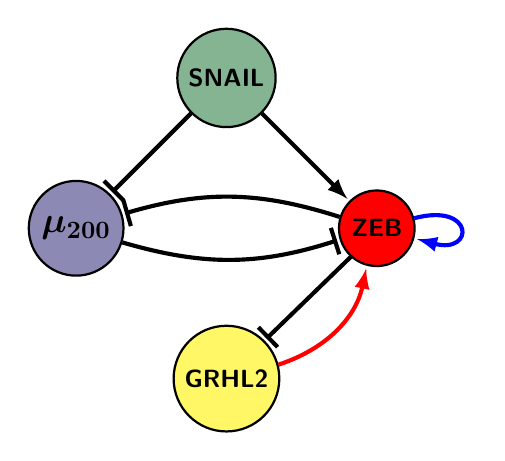
\begin{tikzpicture}[-|, >=stealth', auto, semithick, node distance=3cm,line width = 1.5pt]
\tikzstyle{every state}=[fill=white,draw=black,thick,text=black,scale=0.9]
\node[state, fill=c1]    (snail)                     {\textbf{SNAIL}};
\node[state, fill=c2]    (miR200) [below left of =snail] {\Large{$\boldsymbol{\mu_{200}}$}};
\node[state, fill=c4]    (ZEB)[below right of=snail]   {\textbf{ZEB}};
\node[state, fill=c5] (OVOL) [below left of=ZEB] {\textbf{GRHL2}};
\draw[
    >=latex,
%   every node/.style={above,midway},% either
    auto=right,                      % or
    loop above/.style={out=75,in=105,loop},
    every loop,
    ]
(snail) [-|] edge (miR200)
(snail) [->]edge  (ZEB)
(ZEB) [-|]edge[bend right=17]      (miR200)
(ZEB) edge[loop right, blue] (ZEB)
(OVOL) [->]edge[red] [bend right] (ZEB)
(ZEB) [-|] edge  (OVOL)
(miR200) [-|]edge [bend right=17] (ZEB);
\end{tikzpicture}

\end{figure}

\begin{figure}[!h]
\centering
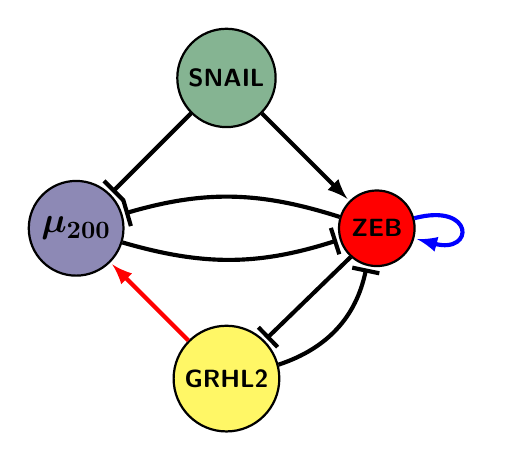
\begin{tikzpicture}[-|, >=stealth', auto, semithick, node distance=3cm,line width = 1.5pt]
\tikzstyle{every state}=[fill=white,draw=black,thick,text=black,scale=0.9]
\node[state, fill=c1]    (snail)                     {\textbf{SNAIL}};
\node[state, fill=c2]    (miR200) [below left of =snail] {\Large{$\boldsymbol{\mu_{200}}$}};
\node[state, fill=c4]    (ZEB)[below right of=snail]   {\textbf{ZEB}};
\node[state, fill=c5] (OVOL) [below left of=ZEB] {\textbf{GRHL2}};
\draw[
    >=latex,
%   every node/.style={above,midway},% either
    auto=right,                      % or
    loop above/.style={out=75,in=105,loop},
    every loop,
    ]
(snail) [-|] edge (miR200)
(snail) [->]edge  (ZEB)
(ZEB) [-|]edge[bend right=17]      (miR200)
(ZEB) edge[loop right, blue] (ZEB)
(OVOL) [-|]edge [bend right] (ZEB)
(ZEB) [-|] edge  (OVOL)
(miR200) [-|]edge [bend right=17] (ZEB)
(OVOL) [->] edge [red] (miR200);
\end{tikzpicture}

\end{figure}


\end{document}